\documentclass[11pt]{article}
\usepackage{float}
%
%Margin - 1 inch on all sides
%
\usepackage[letterpaper]{geometry}
\usepackage{times}
\usepackage{amsmath}
\geometry{top=0.75in, bottom=0.75in, left=0.75in, right=0.75in}

\pagenumbering{gobble}

\usepackage{ragged2e}
\usepackage{mwe}

\usepackage{multicol}

\usepackage{tabularx}

\setlength{\RaggedRightParfillskip}{.25\textwidth plus 1fil}
\setlength{\RaggedRightRightskip}{0pt plus .1\textwidth}
\setlength{\RaggedRightParindent}{1em}


\usepackage{listings}
\usepackage{color}

\definecolor{dkgreen}{rgb}{0,0.6,0}
\definecolor{gray}{rgb}{0.5,0.5,0.5}
\definecolor{mauve}{rgb}{0.58,0,0.82}
\lstset{frame=tb,
    language=c++,
    aboveskip=3mm,
    belowskip=3mm,
    showstringspaces=false,
    columns=flexible,
    basicstyle={\small\ttfamily},
    numbers=none,
    numberstyle=\tiny\color{gray},
    keywordstyle=\color{blue},
    commentstyle=\color{dkgreen},
    stringstyle=\color{mauve},
    breaklines=true,
    breakatwhitespace=true,
    tabsize=3
}

\graphicspath{{../}}

\title{CSCE 451 HW 4}
\author{Benton Guess\{bguess10@tamu.edu\}, Robert Dominguez \{rdominguez@tamu.edu\}}
\date{April 28, 2020}

\begin{document}
\maketitle

\section*{Completed Flags}
We started by playing the game for a while and getting a feel about the types of enemies and stuff that might be important to know about. However, for the sake of time, we only really got out of the original cave and explored a little bit before starting to look into the game.

To begin the reversing process, we did some research on approaches people had previously taken to reversing the game. We found LiveOverflow and a few other posts talking about people who had competed in the challenge. We tried to look at the approaches they had taken without seeing what their solution was (usually just watching the first few minutes of the videos). We did end up getting the entire Mad Cow quest spoiled as well as the existence of the golden eggs, but other than that we didn't see too many other solutions.

The two ideas that came up the most often were binary patches and the symbolic preload method. Using this would mean being able to overwrite functions that ran in the binary. To us, using symbolic preloading seemed to be the most effective since it make a package that could easily be shared between each of us. We also got a cheat engine running for hot patching during the game.

However to begin the symbolic preload method, we needed to recover game classes. From our research, we learned that the \texttt{libGameLogic.so} binary was not stripped, so we began there. We were greeted in IDA with this view.
\begin{figure}[H]
    \centering
    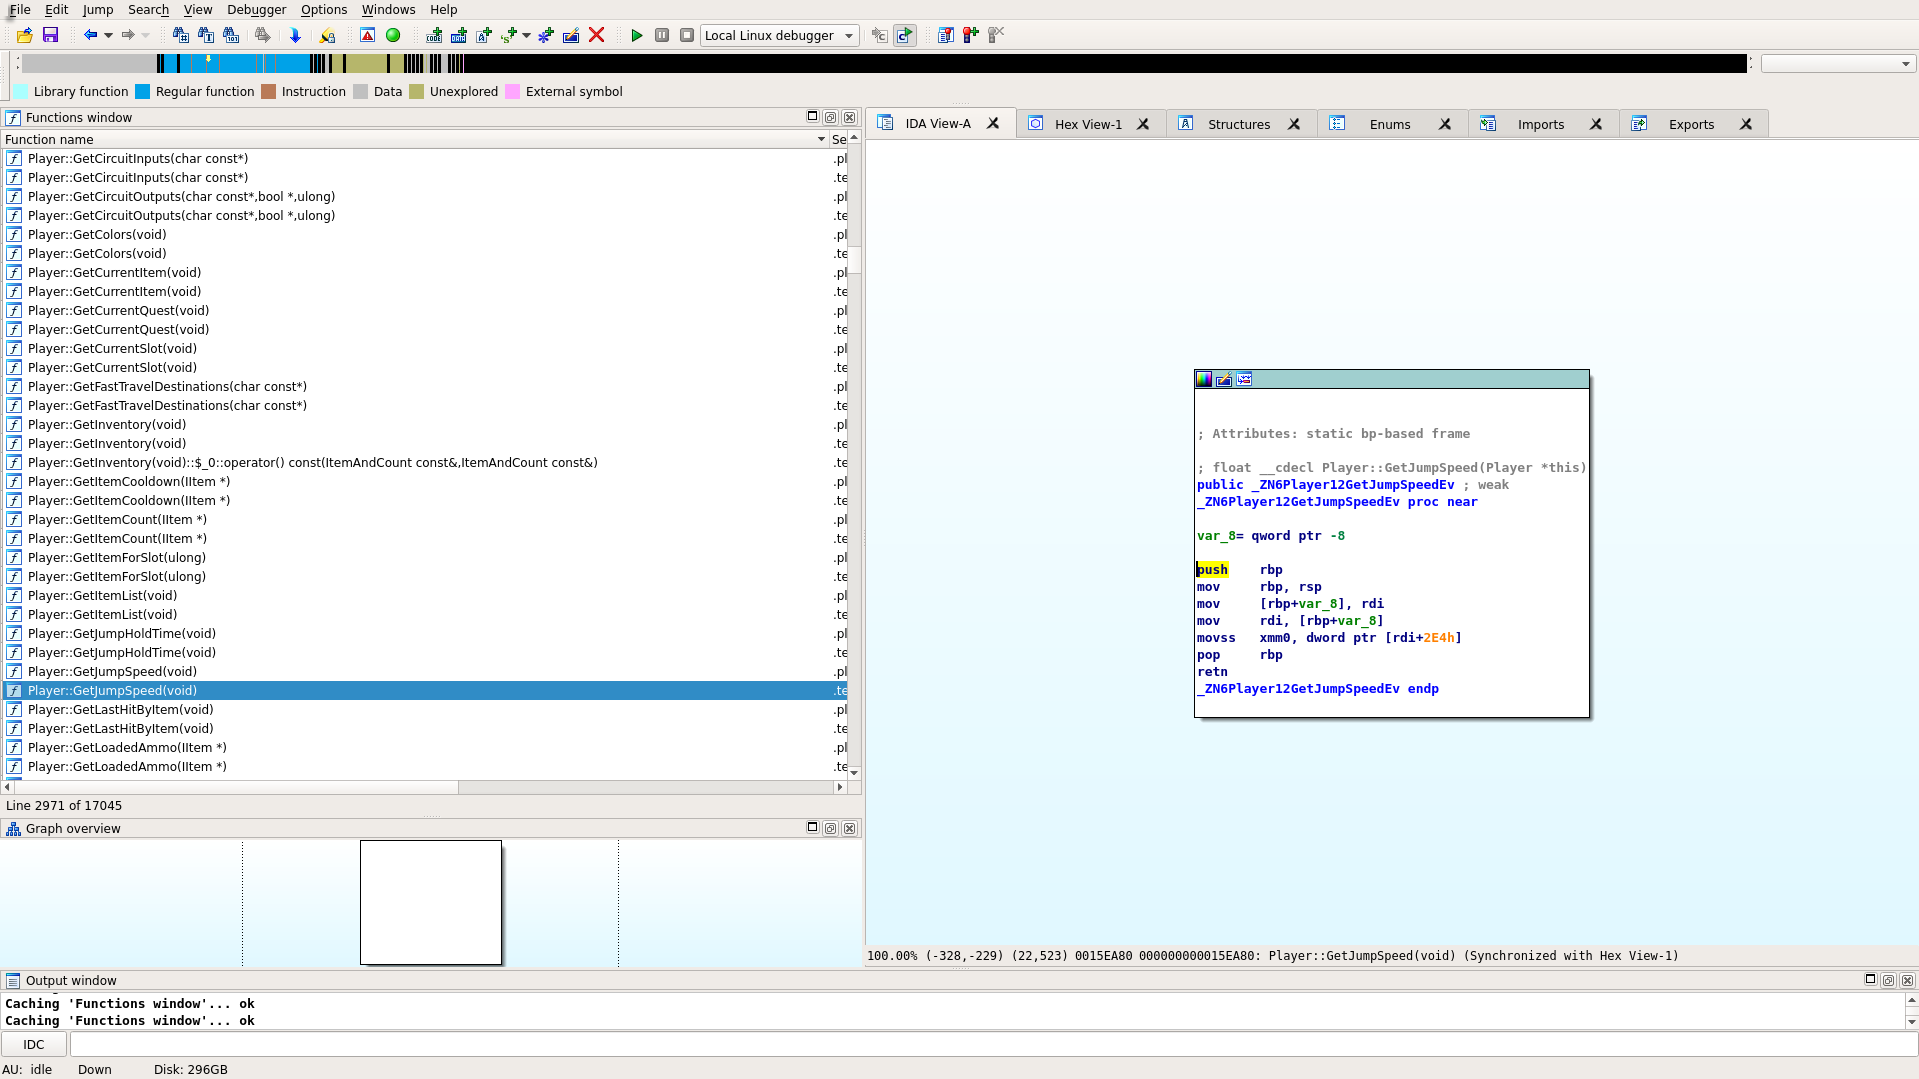
\includegraphics[width=1.00\linewidth]{ida_view.png}
\end{figure}

Here we could easily see that there were many functions controlling things like our jump speed, movement, and position. We decided that the Player class header would be important to recover. Furthermore, we found a few \texttt{Tick} functions that ran inside the game code. Coming from our knowledge of Minecraft, tick functions usually run many times a second, and can be considered continuous functions in terms of the game's timescale. We looked through them to see which ones would be helpful, and found that a few were pretty simple, as in having code inside of them aside from initializing the stack. We then set breakpoints in GDB for a few of the tick functions and found that all of them were running constantly throughout the game. Here we just picked the \texttt{World::Tick} function and decided that we would also want to have access to that though the World header file.

We used GDB to recover the game types, since IDA didn't have an easy function for generating the header files. It took a little bit of time, but it was quite simple to pipe output into files and put them in a directory. The only slight challenge was setting up the order to compile in. This was solved by putting all the headers in a \texttt{pch.h} file and forward declaring nearly all the classes. This ensured that we didnt have to worry about addressing dependencies in any of the files and could just add them to the pch if we found any new ones.
\begin{figure}[H]
    \centering
    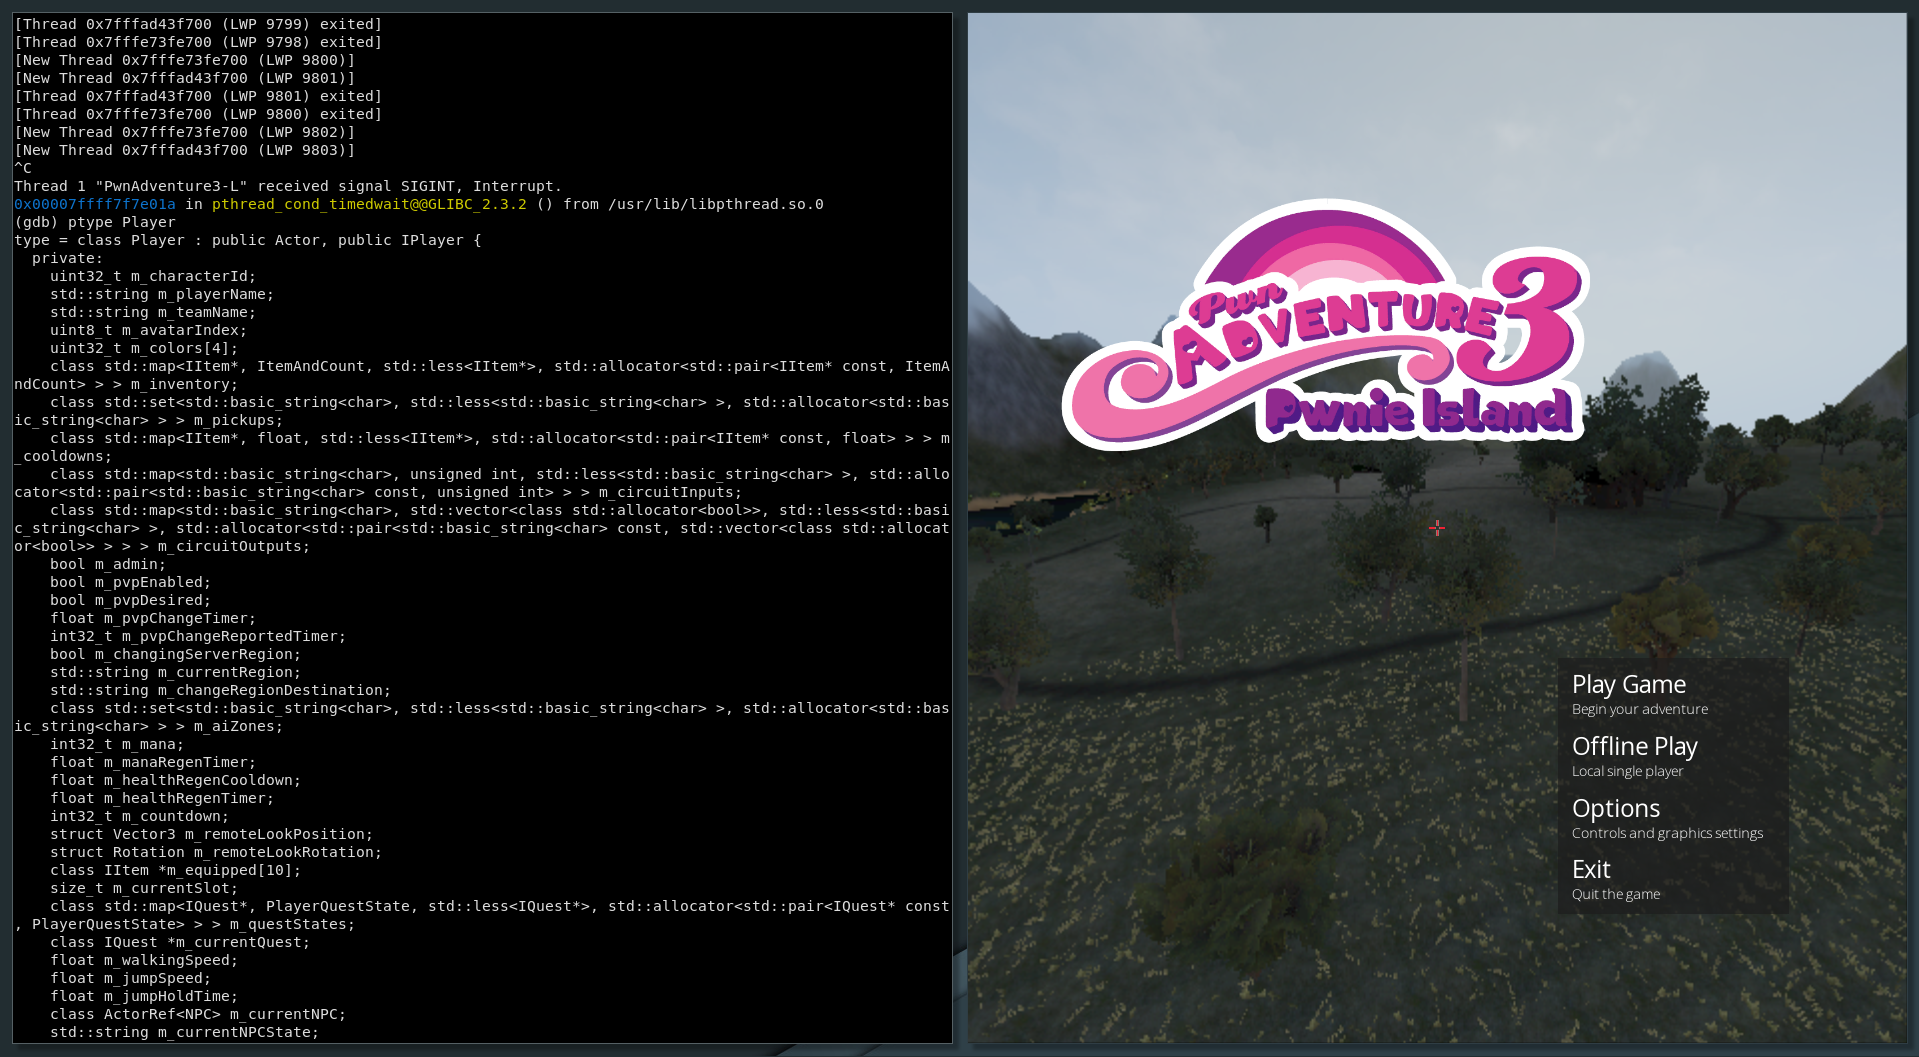
\includegraphics[width=1.00\linewidth]{gdb_ptype.png}
    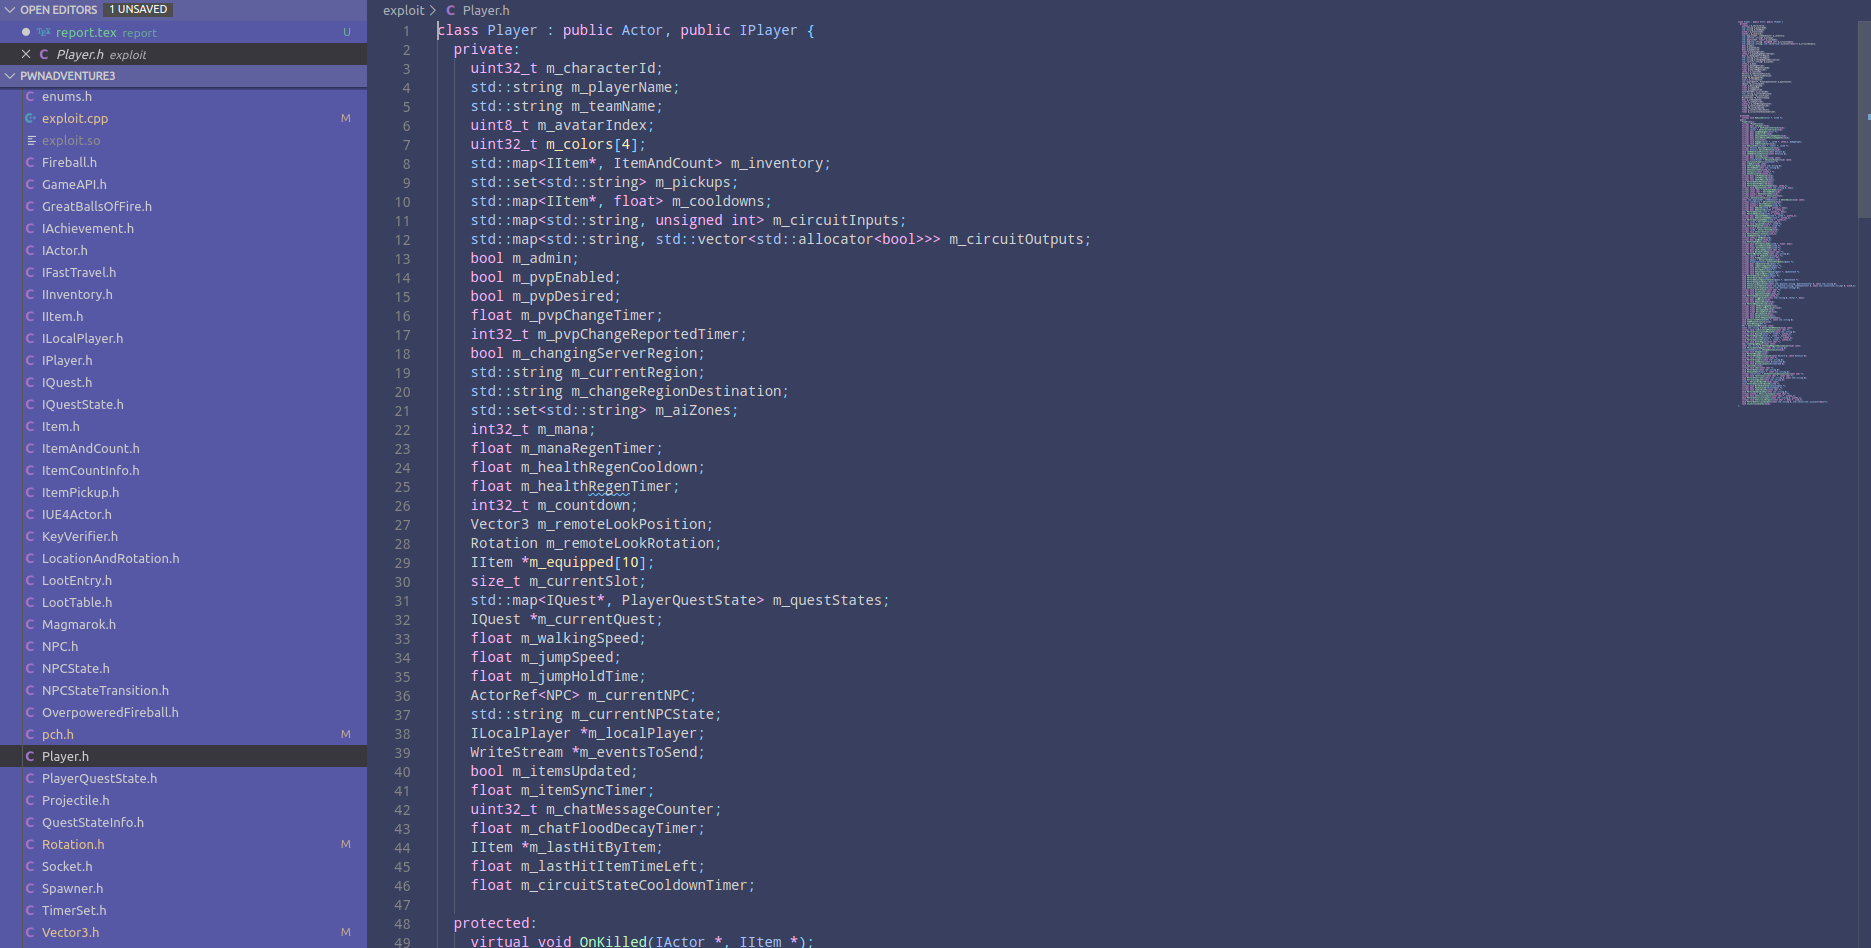
\includegraphics[width=1.00\linewidth]{class_recovery.png}
\end{figure}

We experimented on many of the functions throughout the code to see which ones were running and which we could change (see the pirates DLC section). After that we decided to attempt the challenges.

\subsection*{Mad Cow Flag}

This flag is likely the easiest flag to get in the game, with really no true reversing work needed to finish it. However, we discovered it through reversing work. Once we had loaded the \texttt{LD\_PRELOAD} binary and began experimenting with functions, we found that jump and movement speed were arbitrary overrides that were easy to change. We had already known about there being an island from lookup up information on the game, we just super jumped around until we found the island. We only needed to overload 2 functions through symbolic preload to do this 
\begin{itemize}
    \item \texttt{Player::GetJumpSpeed}
    \item \texttt{Player::GetSprintMultiplier}
\end{itemize}

We talked to the man and got our rubik's cube and killed the cow using static link. However, the chest didn't pop open. We moved on to other challenges in the meantime and came back to it later.

Through the golden egg challenge, we discovered a cow related quest that we were previously unaware of. We realized that it was likely the chest only opened when you killed the cow with the quest active, so we returned to the island using our strategy for finding the golden eggs (which we will explain in that section), killed the cow, and the chest popped open. 
\begin{figure}[H]
    \centering
    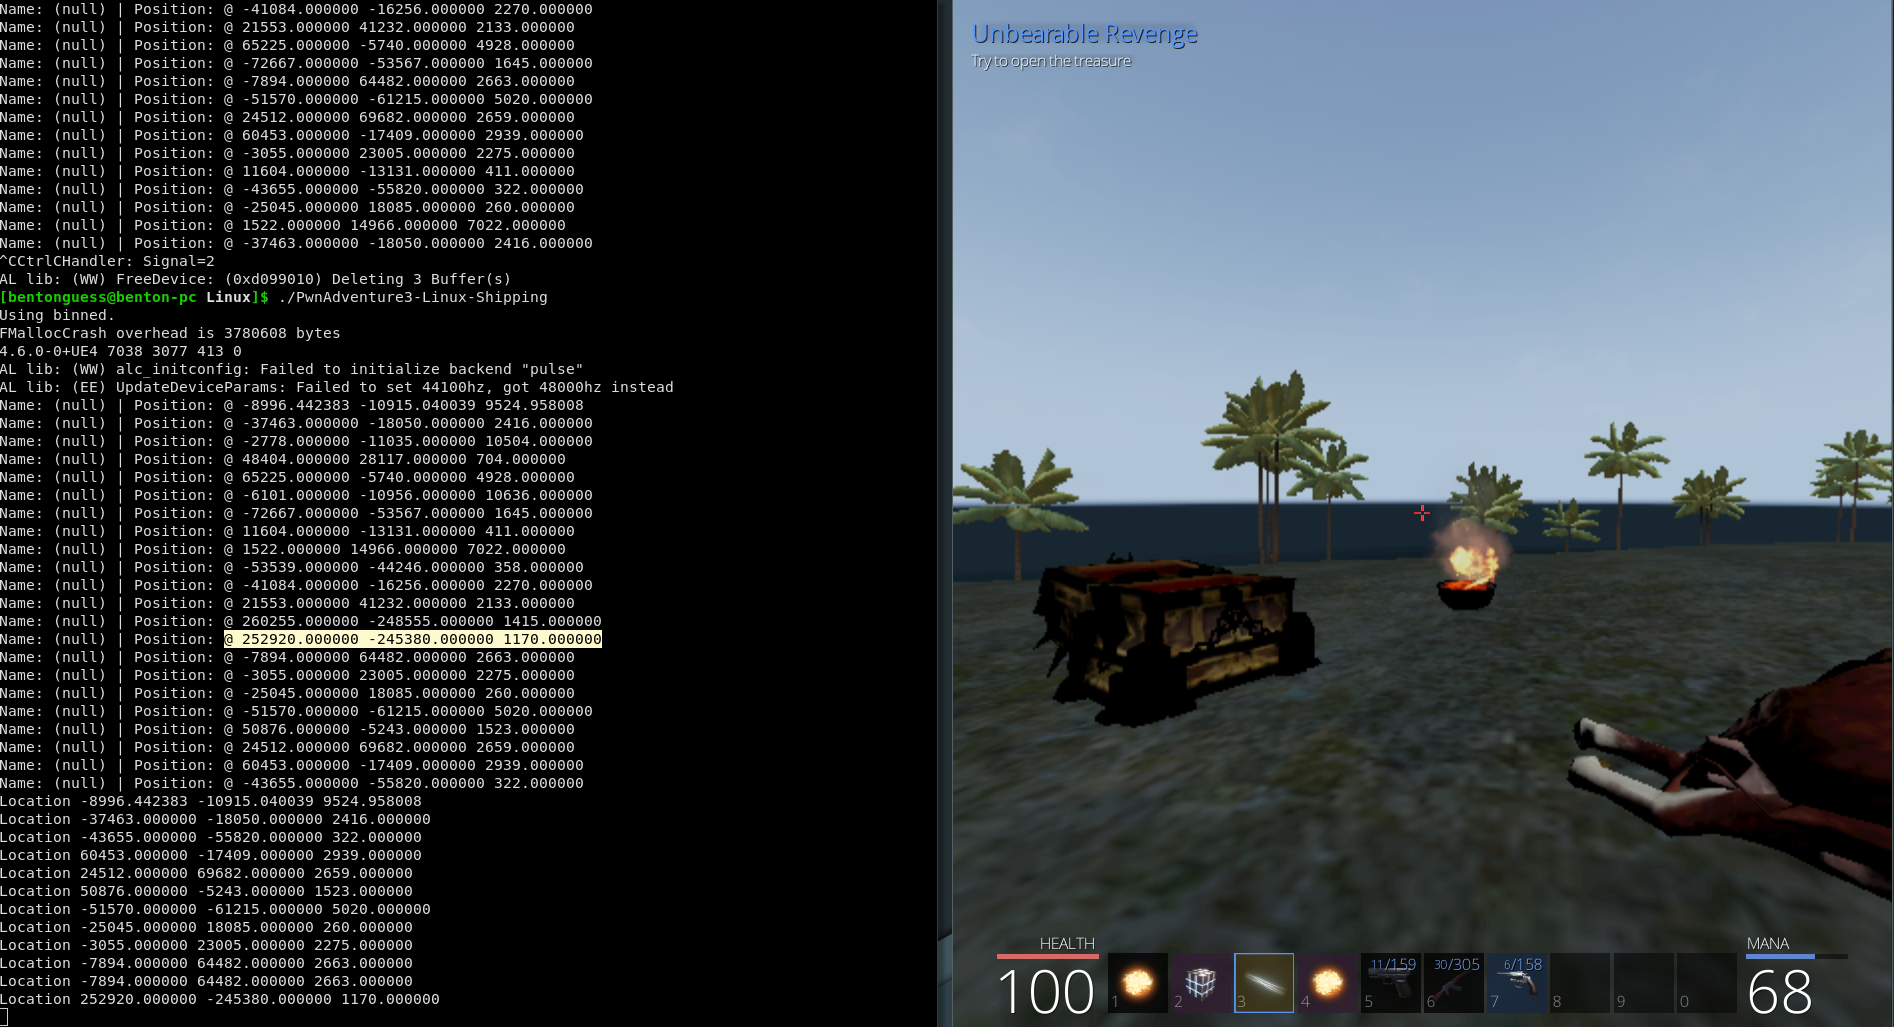
\includegraphics[width=1.00\linewidth]{cow_quest_completed.png}
\end{figure}

\subsection*{Golden Egg Flag}

We had learned about the existence of the golden eggs from our research on the game and decided that finding these would likely be a good place to look for a flag. We looked in IDA to see what would be available, or if the eggs had their own objects, which ended up being the case.

\begin{figure}[H]
    \centering
    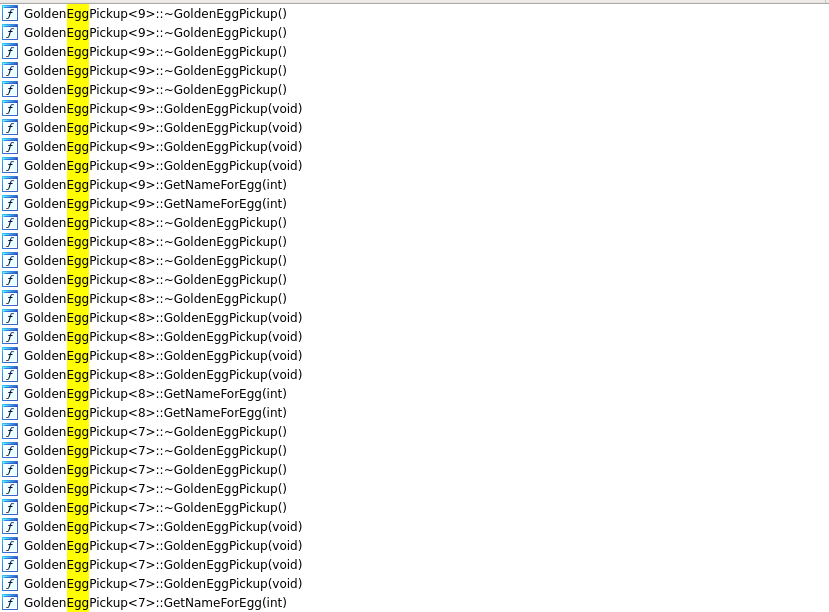
\includegraphics[width=1.00\linewidth]{golden_class.png}
\end{figure}

However, we also found some other object called a \texttt{BallmerEgg}, which we thought probably had something to do with the egg challenge as well. We looked through the only real function it had and found this logic.

\begin{figure}[H]
    \centering
    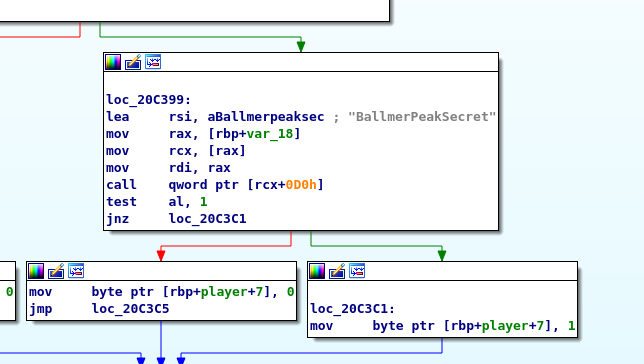
\includegraphics[width=1.00\linewidth]{balmer_peak1.png}
\end{figure}

We found that the \texttt{BallmerEgg::CanUse} function had this logic in it regarding a secret phrase or something like that. It looked like it directly made the egg usable, based on the branch condition. The code likely looked something like this: 
\begin{lstlisting}
    bool cond = this->GetValueBasedOnString("BallmerPeakSecret");
    if (cond) {
        player->b_some_var = true;
    } else {
        player->b_some_var = false;
    }
\end{lstlisting}

We XREFed the string and found that another function used it, and was associated with a \texttt{BallmerPoster::Damage} function.

\begin{figure}[H]
    \centering
    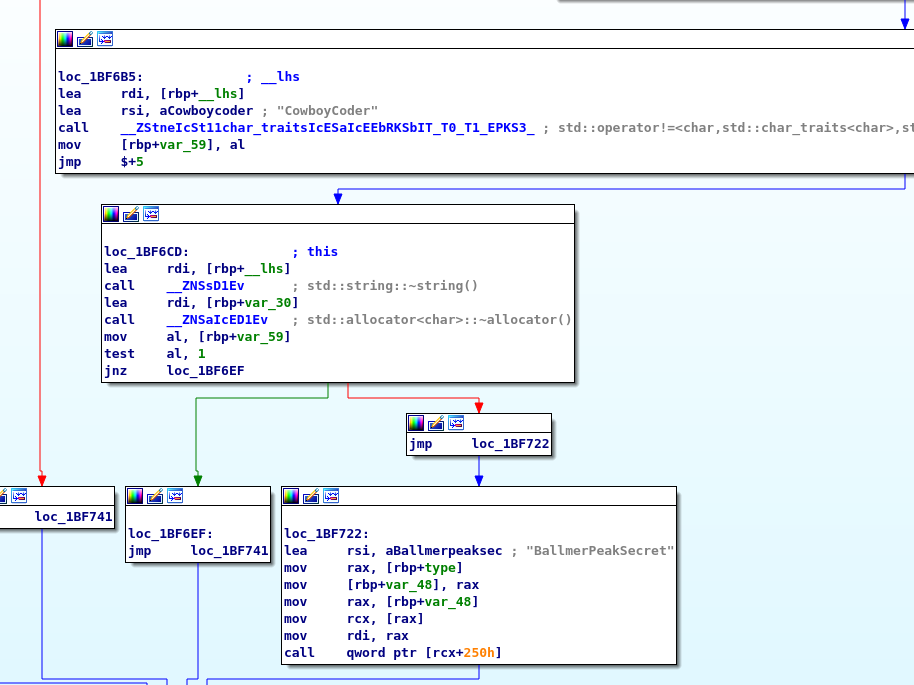
\includegraphics[width=1.00\linewidth]{balmer_peak2.png}
\end{figure}

We found a snippet of code basically saying this

\begin{lstlisting}
    if ("CowboyCoder" != _some_string_) {
        continue;
    } else {
        // it looks like its calling a static function from the DamageType enum?
        // This could be an IDA error, or we just dont understand something in the function
        // Regardless, this is a "smoking gun" (no pun intended) that we think is doing something important
        type->SomeFunction(..., "BalmerPeakSecret");
    }
\end{lstlisting}

This made us think that whatever this enemy was, damaging them with a Cowboy Coder did something to make the egg usable. So we guessed that finding this enemy and killing them would make the egg usable. However, due to some other reversing work we did, we didn't have to worry about finding them.

As we began looking through the game code for metadata we could use, we found that two \texttt{std::set} variables were being stored in World. One of us wanted to be able to see other players on the map (for the future multiplayer hack). We found with cheat engine that there was a place in the code where all the other players locations are stored, along with the NPC's. The first candidate was the game world class whose \texttt{Tick} function we had grabbed earlier. Here we found two variables that could be used.

\begin{itemize}
    \item \texttt{m\_players}
    \item \texttt{m\_actors}
\end{itemize}

We initially tried using the \texttt{m\_players} set, however, this was somewhat difficult to extract the locations, and there were many null pointers to wade through, so we tried the \texttt{m\_actors} variable instead, which was much easier to tame. This simple peice of code allowed us to print all the actors. We overrode the chat function (something we had picked up from LiveOverflow's videos) so that we could type "A" and print this entire map. The code was as follows occured inside the \texttt{World::Tick} function.

\begin{lstlisting}
    // we set print_all_actors global variable in a chat command by overriding the chat function
    if (print_all_actors) {
        print_all_actors = false;

        for (const ActorRef<IActor>& actor_ref: this->m_actors) {
            Actor* actor = (Actor*)actor_ref.Get();
            Vector3 position = actor->GetPosition();
            const char* name = actor->GetDisplayName();
            printf("Name: %s | Position: @ %f %f %f\r\n", name, position.x, position.y, position.z); 
        }
    }
\end{lstlisting}

Using the actors set was actually better, since nearly every class within the game is derivative of \texttt{Actor}.

One of us immediately started teleporting around, using another chat command we had written to modify the player location, and found one of the eggs.

\begin{figure}[H]
    \centering
    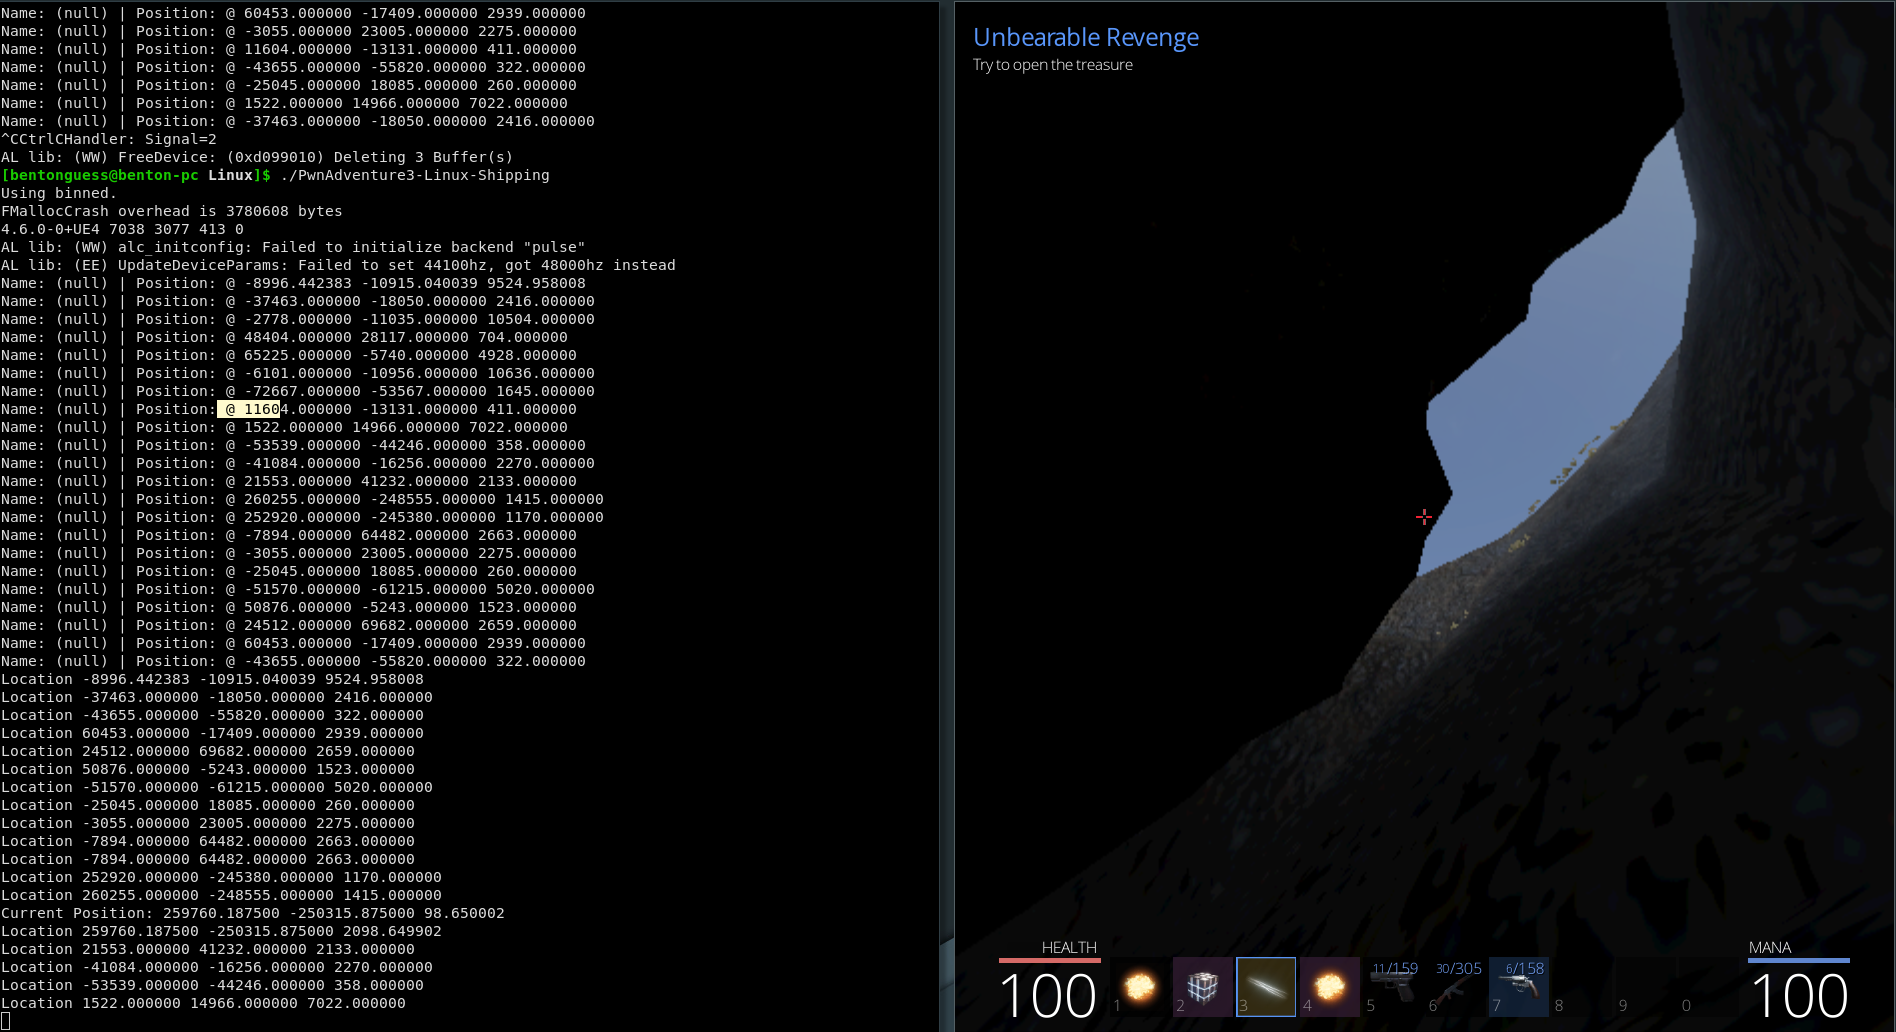
\includegraphics[width=1.00\linewidth]{golden_egg2.png}
\end{figure}

Quite a terrible location to be, since you're pretty much soft locked down there. Regardless, we ended up finding the entire suite of eggs this way, but midway through our teleportation quest, we found this. 
\begin{figure}[H]
    \centering
    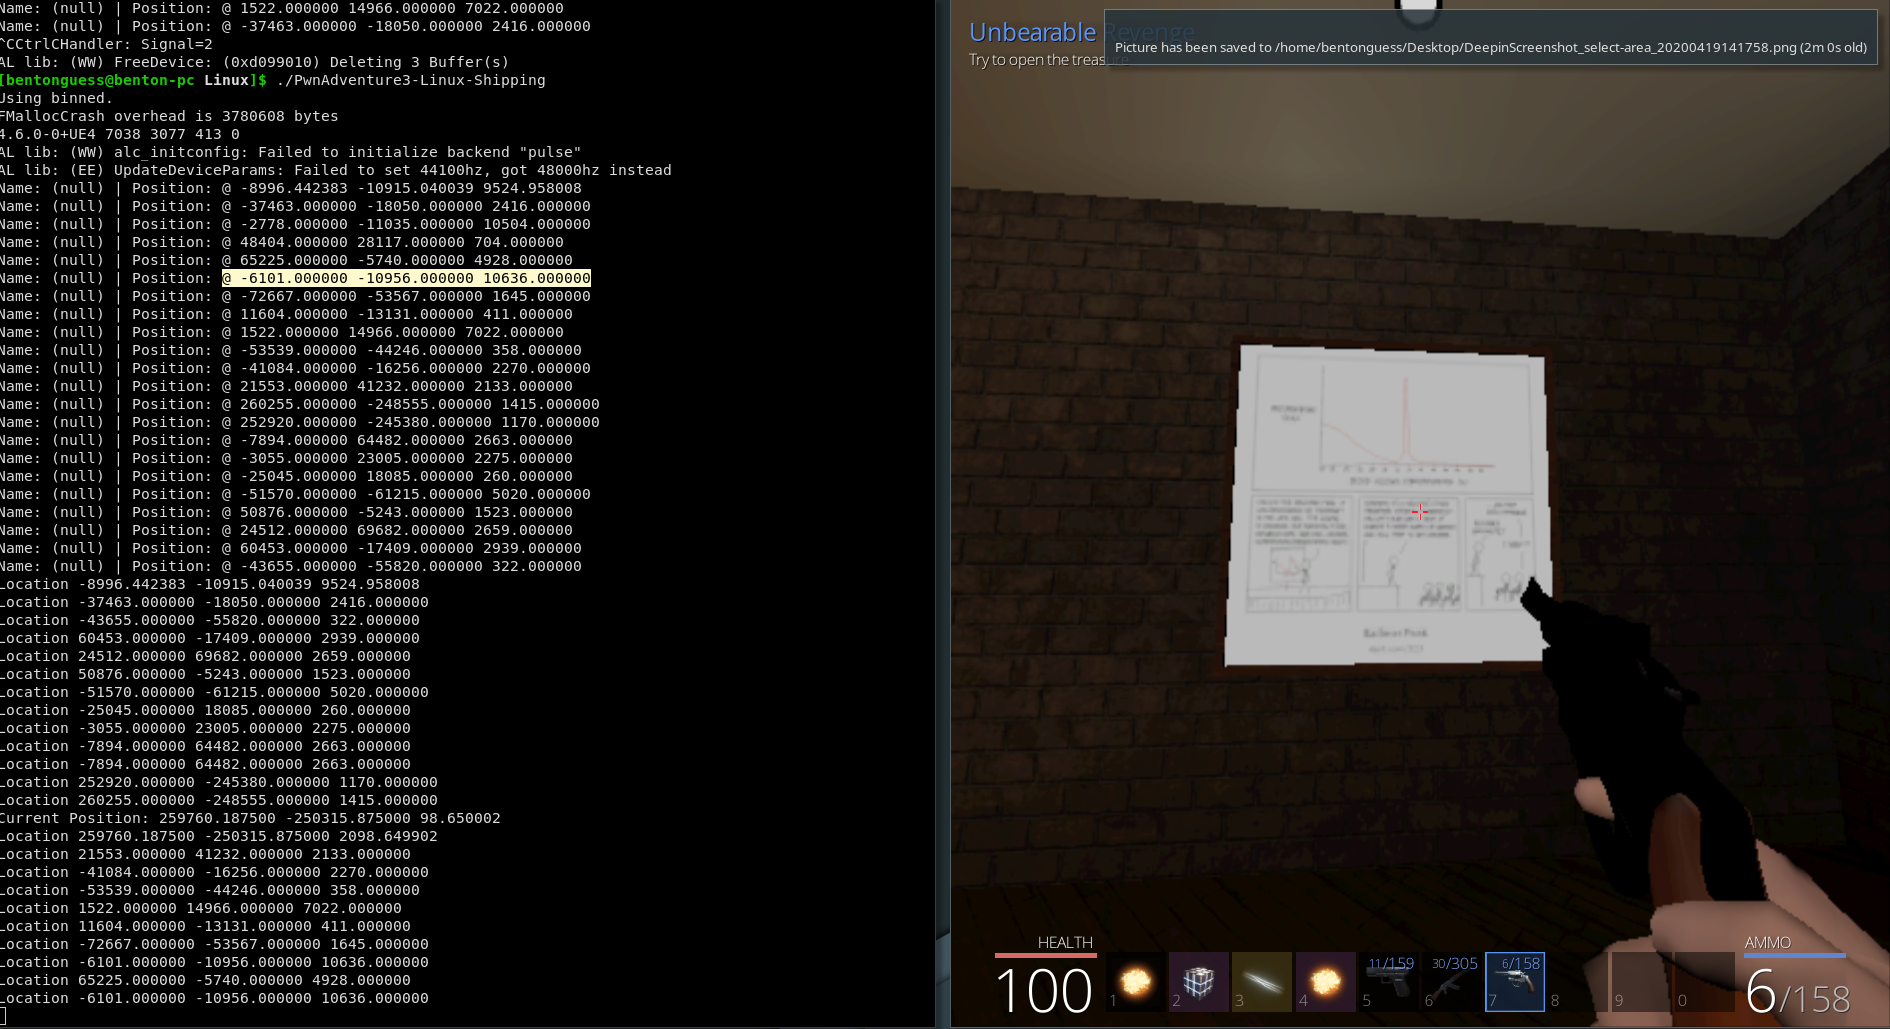
\includegraphics[width=1.00\linewidth]{shoot_poster.png}
\end{figure}

We realized that our location at the moment was Ballmer Peak, and we realized that this was the legendary boss we had found earlier in he games code that could only be killed with the cowboy coder. We shot it and nothing happened. We had thought that the exploit we had found didn't work, but in the end it actually did. After a few more rounds of teleporting through the map, we appeared at Ballmer peak in front of an egg on the deck. One of us then verified that, yes, if you don't shoot the poster, the egg will not appear.

From there we had our second flag and a list of new locations to go to.

\subsection*{Bear Chest Flag}

While teleporting around, we found this terrible place where a chest was guarded by bears and touching it essentially started a bear war. We thought that the best way to solve this would be to modify the player class stats and just make yourself a god, un-killable by bears. However, as we had learned earlier, our powers were limited to location, speed, and jump, along with viewing the games variables. We tried to modify things like mana and health again but we still couldn't find a way to deal with the bears that way. Jumping didn't work, as the bears would eventually fill the entire space and you couldn't move. 

We then tried holding a constant position in the air where the bears couldn't get us. However, we were couldn't go too high, and the bears could still damage us while floating. This told us that the hitboxes in this game were pretty buggy, or at least the way that the bears attacked. Finally, we tried to wedge ourselves in the tree with jump, but we could stay stable in a tree for more than a few seconds at a time.

We settled on using our location to clip into the chest and a little underground so that the bears couldnt attack us, as we found that unlike the air, underground was pretty safe from bears.

We made this code to clip us into the ground/chest.

\begin{lstlisting}
// Occurs within the overriden chat function
if (str[0] == 'H') {
    b_hold_position = true;
    v_hold_position = position;
}
else if (str[0] == 'h') {
    b_hold_position = false;
}
else if (str[0] == 'D') {
    position.z -= 100;
    v_hold_position = position;
} 
... 
// Occurs within the World::Tick function
// We initialize these in the chat function
bool b_hold_position = false;
Vector3 v_hold_position;
Player* me
...
void World::Tick(...) {
    ...
    if (b_hold_position) {
        me->SetPosition(v_hold_position);
    }
    ...
}
\end{lstlisting}

This worked, but some spots under the chest would have you failing the challenge by leaving the area. We assumed this had to do with the fact that being underground probably caused the game's logic to spaz out, and you would just randomly fail the challenge. However, we found that when we used the function to hold, then clipped through the ground on the edge of the back of the chest by about give or take 400 units, it worked consistently for running the five minutes down.

\section*{Attempted (but Failed) Flags}

\subsection*{"Block" Flag}

\begin{figure}[H]
    \centering
    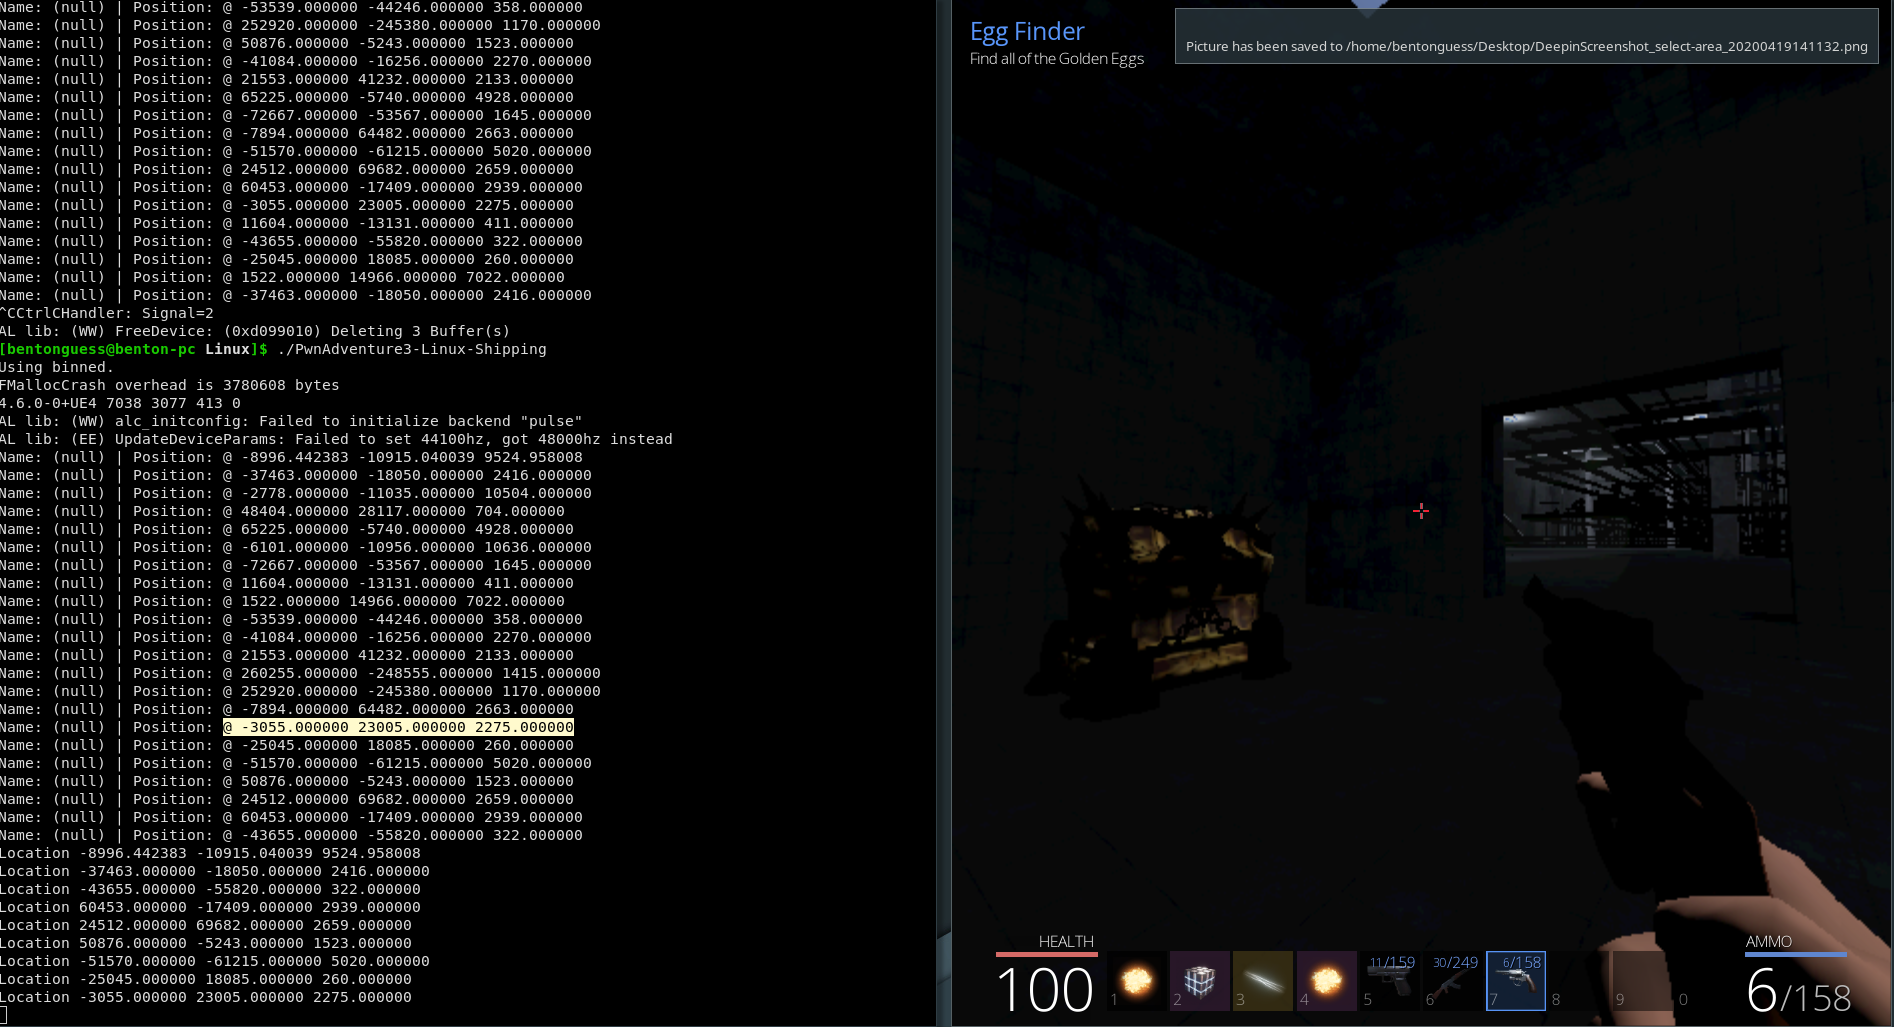
\includegraphics[width=1.00\linewidth]{block.png}
\end{figure}

We called this the "block" flag since when we looked into the games code, we found that the flag was called using the text string "block" in the games code. We found this during our search for the golden eggs. Upon exploration, its some underground room that we never found while roaming the map, and it may not even be accessible from the outside anywhere. Initially, we teleported into the chest room for this challenge and found that the puzzle was a circuit that essentially encoded some form of password in 32 bit form. Our intuition was that the circuit was being simulated through some function in code We made some initial attempts at this by looking through the code in IDA, however we were not able to find any piece of code that directly handled the logic of this function. From here we decided that the only two options was that the circuit was being simulated in some stripped function, or that the code was quite literally being simulated through the physics engine. Both ways, this would have to be a brute force that we put aside. Another option would be to transcribe the logic gates into a manner that could be simulated either with brute force or through something like Z3, however this was also going to be much too time consuming.

\subsection*{Pirate DLC Flag and Magmarok Flag}

\begin{figure}[H]
    \centering
    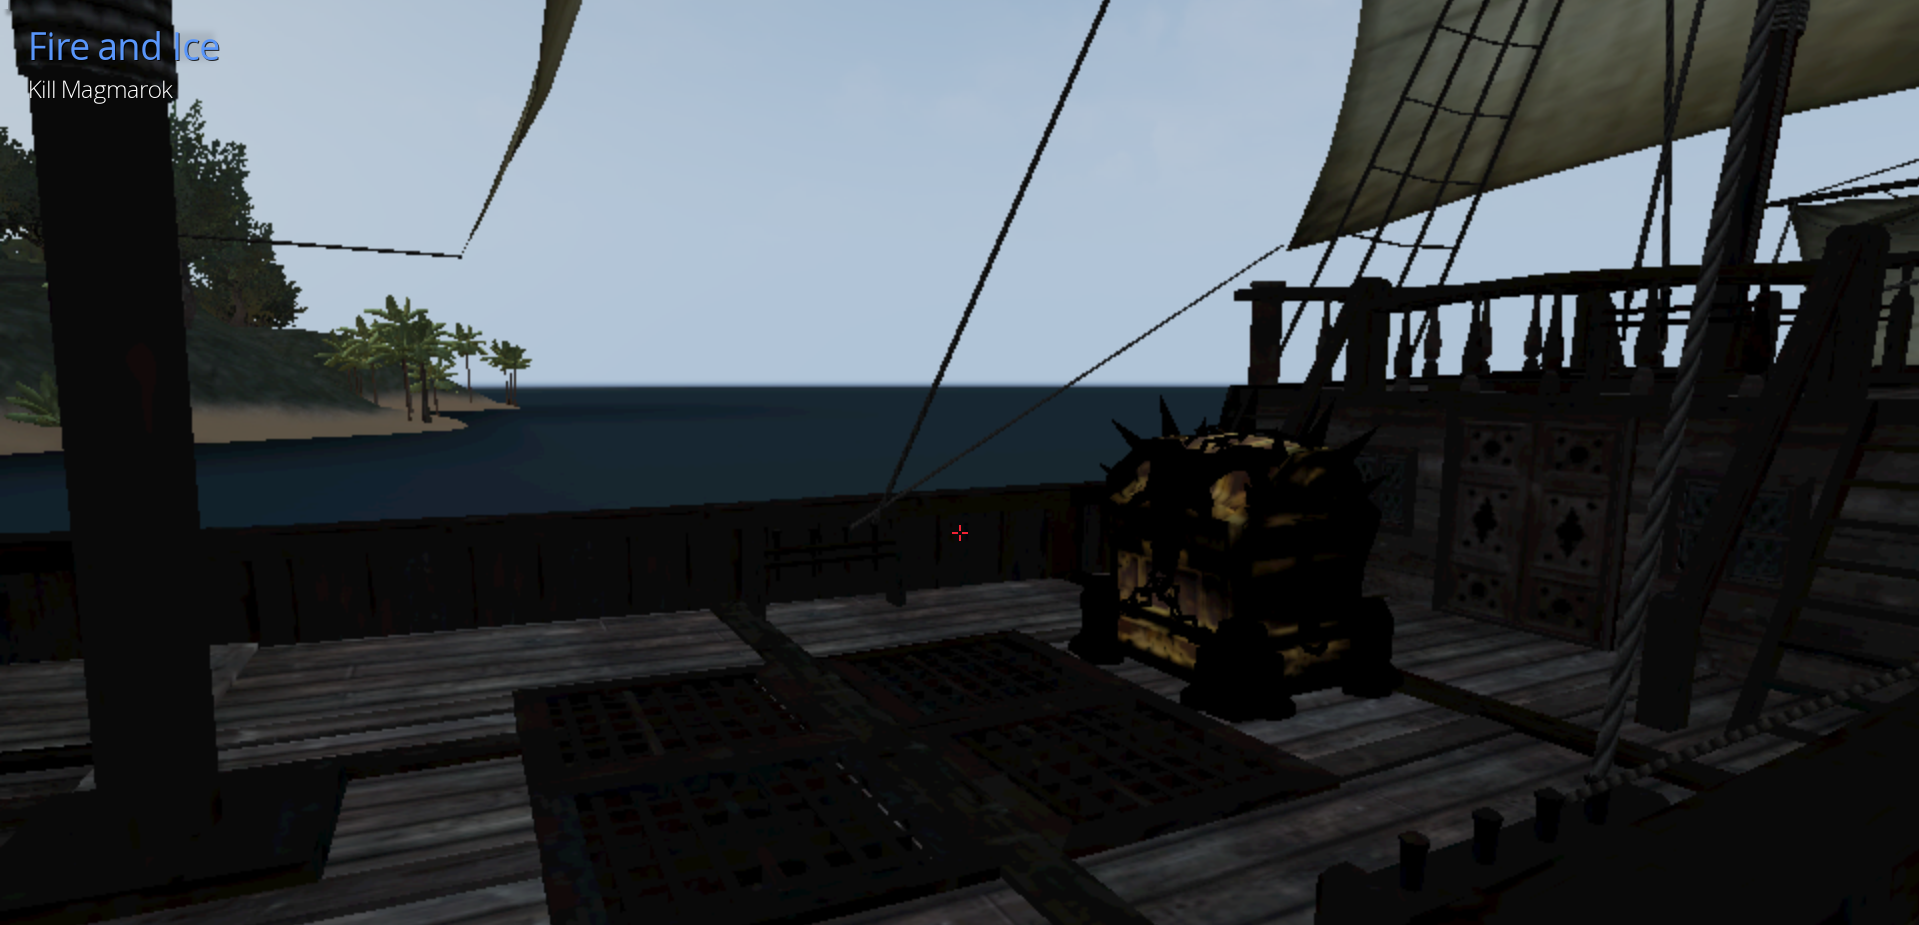
\includegraphics[width=1.00\linewidth]{pirate.png}
    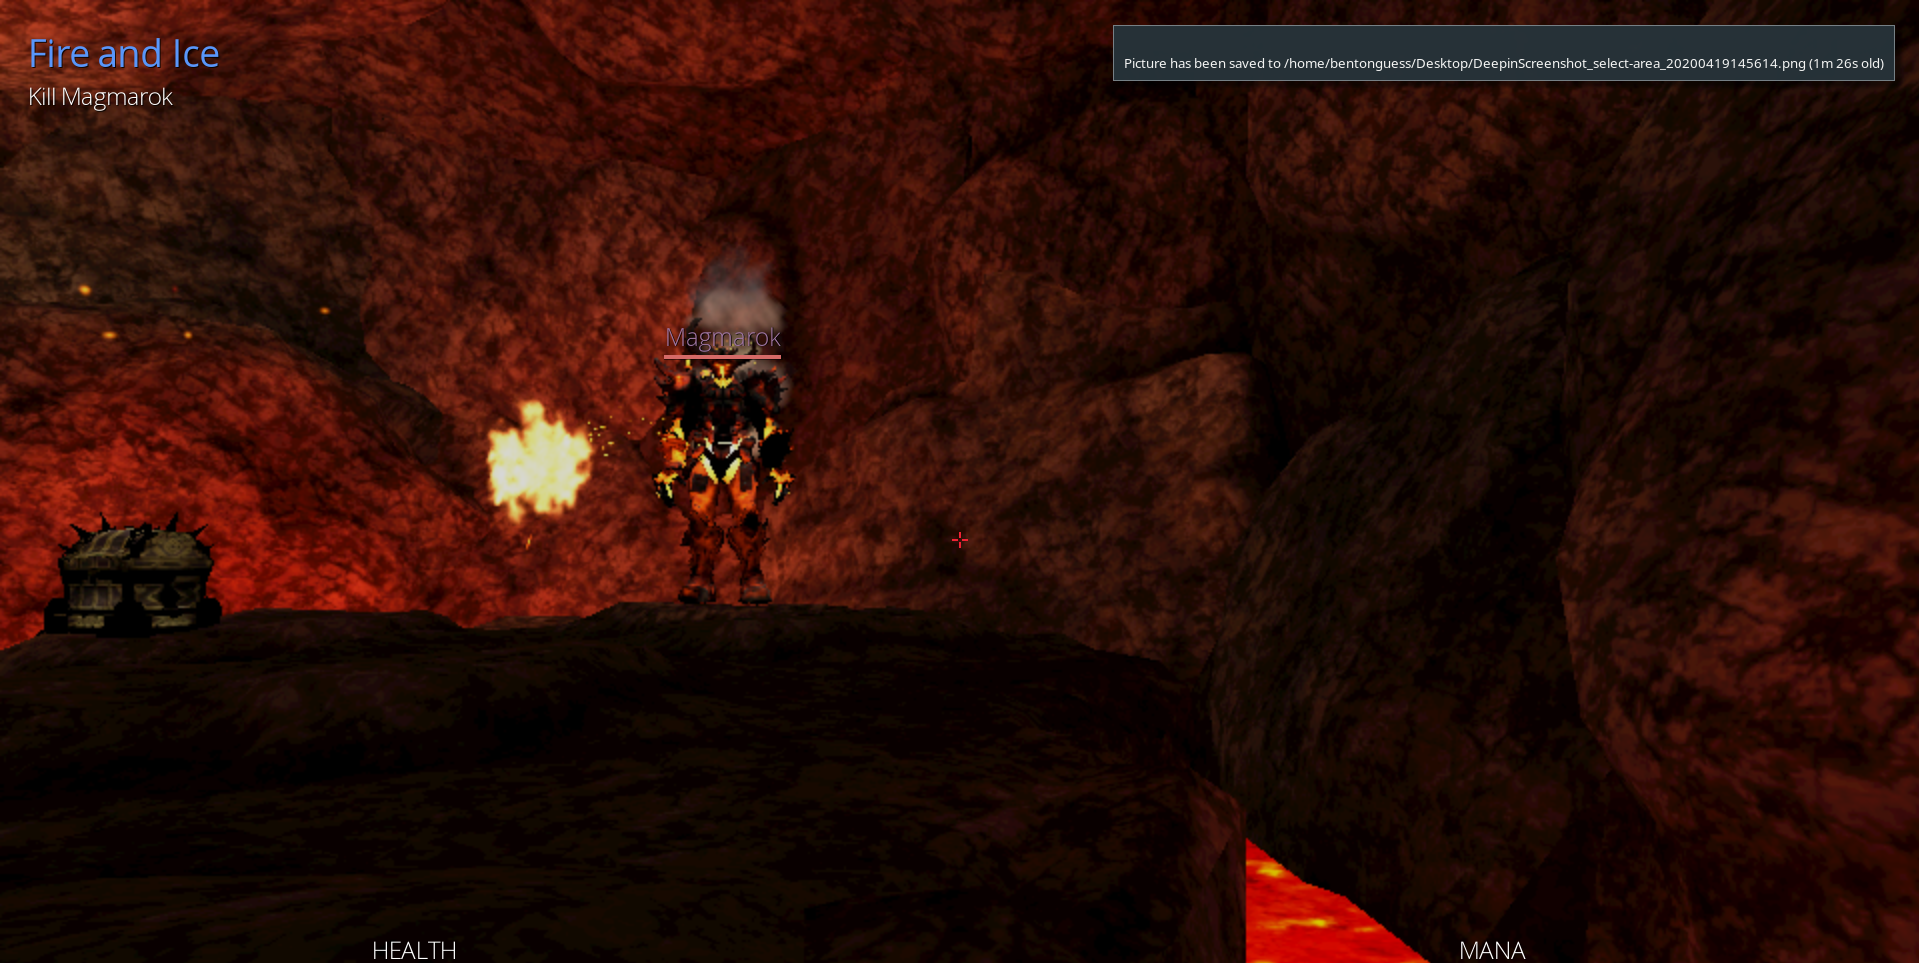
\includegraphics[width=1.00\linewidth]{magmarok.png}
\end{figure}

These were the first two flags we attempted to solve since it was the first chest we came across. We assumed that the chest would simply have a function that we could overwrite through preloading. However, after many attempts to overwrite this function and trigger an opened chest, we found that the preload method was not sufficient to open this chest, and the key function itself had to be reversed. However, this actually was our most important experience while getting a flag, as it taught us some of the more important things to know about the binary
\begin{itemize}
    \item There were functions that were likely being only run server side, indicating that the \texttt{libGameLogic.so} was being shared between client and server
    \item The only editable values on Player were the location and other positional data
    \item The World class had a tick function that was empty but still running every time.
    \item The general hierarchy of Player -> Actor -> IActor etc when it came to the game classes
\end{itemize}

After we gave up on trying to solve the pirate DLC, we moved onto the next chest we found, Magmarok. Here we tried things like increasing the damage on our weapons, giving ourselves more mana and health, and trying to modify the functions that were controlling Magmarok to no avail. Ultimately we decided that there were only a small sliver of functions that the server wasn't constantly validating, and making sure we took advantage of those would be incredibly important. 

Robert tried to work on the boss for longer with a cheat engine rather than a preloader, but this was only able to damage him to a point where he would heal himself instantly. We also set Magmarok aside since it was just going to be too time consuming to try and beat him.

\section*{Multiplayer Exploit}
The tools we had already created for getting flags were actually sufficient to give us a serious advantage in multiplayer.First off, we have a function that gives us a look into the list of currently online actors, and we can tell who the players are by looking for coordinates with a decimal value. 
\begin{lstlisting}
    Name: (null) | Position: @ -34837.542969 -17287.904297 2500.787598
    Name: (null) | Position: @ -44670.308594 -4952.907715 1905.776733
    Name: (null) | Position: @ -12576.258789 -57224.339844 3194.650635
    Name: (null) | Position: @ -72667.000000 -53567.000000 1645.000000
    Name: (null) | Position: @ -2778.000000 -11035.000000 10504.000000
    Name: (null) | Position: @ 65225.000000 -5740.000000 4928.000000
    Name: (null) | Position: @ 48404.000000 28117.000000 704.000000
    Name: (null) | Position: @ 11604.000000 -13131.000000 411.000000
    Name: (null) | Position: @ 1522.000000 14966.000000 7022.000000
    Name: (null) | Position: @ 21553.000000 41232.000000 2133.000000
    Name: (null) | Position: @ 260255.000000 -248555.000000 1415.000000
    Name: (null) | Position: @ -53539.000000 -44246.000000 358.000000
    Name: (null) | Position: @ -41084.000000 -16256.000000 2270.000000
    Name: (null) | Position: @ -43655.000000 -55820.000000 322.000000
    Name: (null) | Position: @ -25045.000000 18085.000000 260.000000
    Name: (null) | Position: @ -51570.000000 -61215.000000 5020.000000
    Name: (null) | Position: @ 24512.000000 69682.000000 2659.000000
    Name: (null) | Position: @ 252920.000000 -245380.000000 1170.000000
    Name: (null) | Position: @ 50876.000000 -5243.000000 1523.000000
    Name: (null) | Position: @ -3055.000000 23005.000000 2275.000000
    Name: (null) | Position: @ -7894.000000 64482.000000 2663.000000
    Name: (null) | Position: @ 60453.000000 -17409.000000 2939.000000
    Name: (null) | Position: @ -37463.000000 -18050.000000 2416.000000
    Name: (null) | Position: @ -6101.000000 -10956.000000 10636.000000
\end{lstlisting}

We also have a teleport function, which is called by placing an \texttt{@} symbol as the first character in chat, then giving three coordinates. As you can see, this is the same format the actors are reported in. From here we had worked out the very simple math it would take to implement an aimbot. However, no matter what functions we overrode through our preload injection, we could not find a sufficient method to alter the players FOV rotation. I assume this has to do with the input API being obfuscated and overriding our wishes. Still, with a player list and and a teleport, we could give ourselves a significant multiplayer advantage.

We added a command to the chat interceptor, \texttt{Q}, that would down warp the player. The combination of these three tools and giving ourselves a very high jump meant that we could easily perform a "stealth" kill. We can easily look at the list of players, then grab a name (the first one is always you), and set your z coordinate to zero. This will put you under a player, looking up from them in a clear floor. The injection also gives you a super jump and super speed, so all you need to do from there is jump, and you will clip above the ground wherever you please, for a quick assassination. There are also even some places in the ground textures where collisions do not get detected, so you could even shoot them from below.
\end{document}